\documentclass{standalone}
\usepackage{tikz}
\usetikzlibrary{patterns, positioning}
\usepackage[sfdefault]{ClearSans} %% option 'sfdefault' activates Clear Sans as the default text font
\usepackage[T1]{fontenc}

\begin{document}
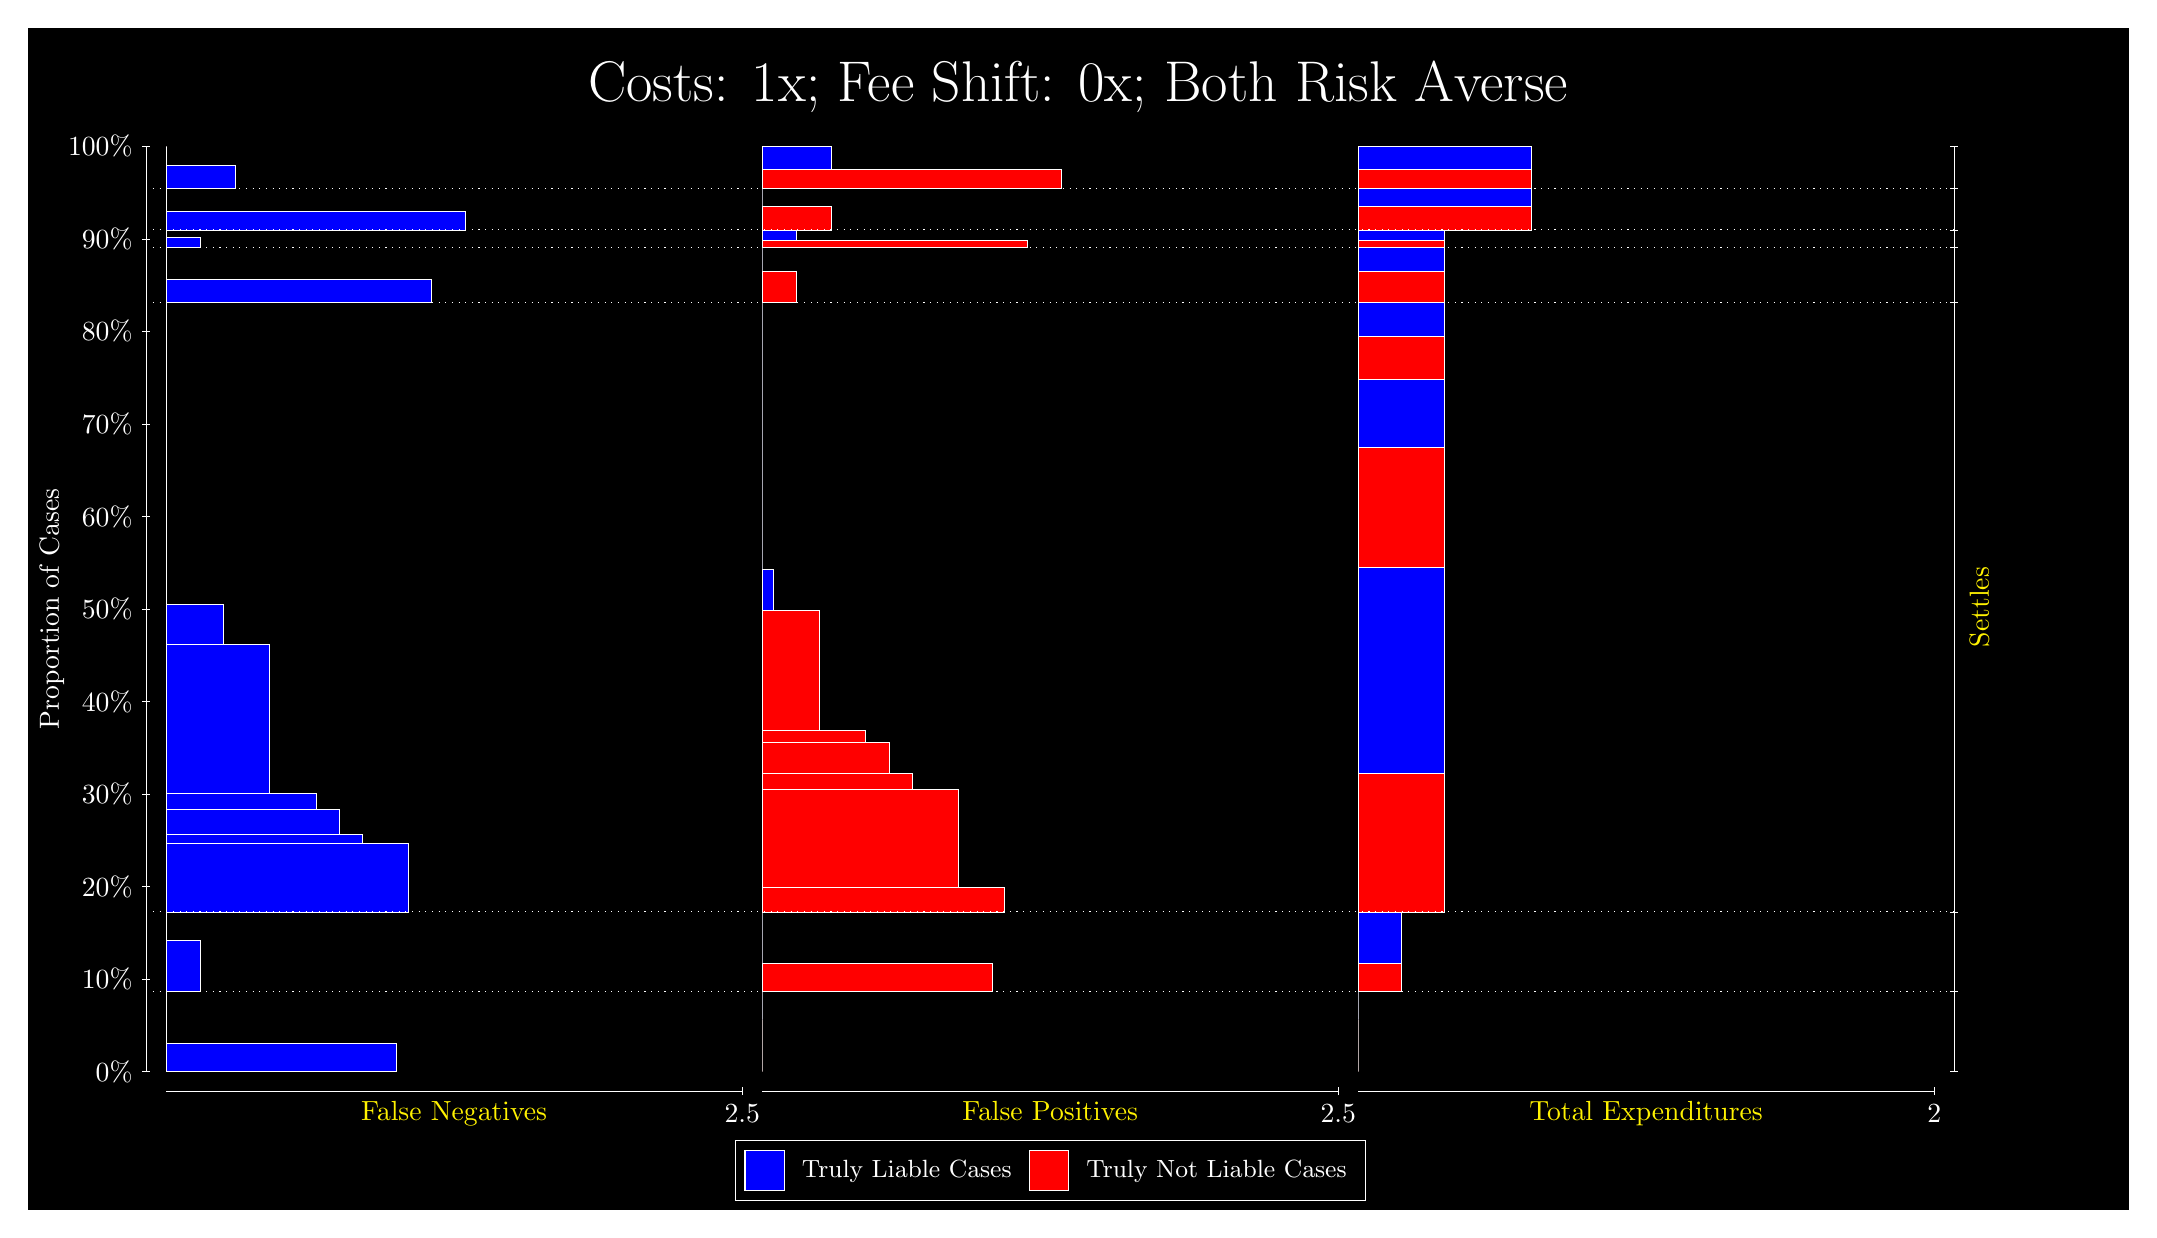
\begin{tikzpicture}
\draw[fill=black] (0,0) rectangle (26.667,15);
\draw[text=white] (0,13.5) rectangle (26.667,15) node[midway] {\huge Costs: 1x; Fee Shift: 0x; Both Risk Averse};
\draw[white, very thin] (1.5,1.75) -- (1.5,13.5);
\node[rotate=90, text=white, anchor=center] at (0.3, 7.625) {Proportion of Cases};
\draw[white, very thin] (1.45,1.75) -- (1.55,1.75);
\node[text=white, anchor=east] at (1.45, 1.75) {0\%};
\draw[white, very thin] (1.45,2.925) -- (1.55,2.925);
\node[text=white, anchor=east] at (1.45, 2.925) {10\%};
\draw[white, very thin] (1.45,4.1) -- (1.55,4.1);
\node[text=white, anchor=east] at (1.45, 4.1) {20\%};
\draw[white, very thin] (1.45,5.275) -- (1.55,5.275);
\node[text=white, anchor=east] at (1.45, 5.275) {30\%};
\draw[white, very thin] (1.45,6.45) -- (1.55,6.45);
\node[text=white, anchor=east] at (1.45, 6.45) {40\%};
\draw[white, very thin] (1.45,7.625) -- (1.55,7.625);
\node[text=white, anchor=east] at (1.45, 7.625) {50\%};
\draw[white, very thin] (1.45,8.8) -- (1.55,8.8);
\node[text=white, anchor=east] at (1.45, 8.8) {60\%};
\draw[white, very thin] (1.45,9.975) -- (1.55,9.975);
\node[text=white, anchor=east] at (1.45, 9.975) {70\%};
\draw[white, very thin] (1.45,11.15) -- (1.55,11.15);
\node[text=white, anchor=east] at (1.45, 11.15) {80\%};
\draw[white, very thin] (1.45,12.325) -- (1.55,12.325);
\node[text=white, anchor=east] at (1.45, 12.325) {90\%};
\draw[white, very thin] (1.45,13.5) -- (1.55,13.5);
\node[text=white, anchor=east] at (1.45, 13.5) {100\%};

\draw[white, very thin] (24.457,1.75) -- (24.457,13.5);
\draw[white, very thin] (24.407,1.75) -- (24.507,1.75);
\node[anchor=west] at (24.407, 1.75) {};
\draw[white, very thin] (24.407,2.7678) -- (24.507,2.7678);
\node[anchor=west] at (24.407, 2.7678) {};
\draw[white, very thin] (24.407,3.7767) -- (24.507,3.7767);
\node[anchor=west] at (24.407, 3.7767) {};
\draw[white, very thin] (24.407,11.521) -- (24.507,11.521);
\node[anchor=west] at (24.407, 11.521) {};
\draw[white, very thin] (24.407,12.213) -- (24.507,12.213);
\node[anchor=west] at (24.407, 12.213) {};
\draw[white, very thin] (24.407,12.44) -- (24.507,12.44);
\node[anchor=west] at (24.407, 12.44) {};
\draw[white, very thin] (24.407,12.97) -- (24.507,12.97);
\node[anchor=west] at (24.407, 12.97) {};
\draw[white, very thin] (24.407,13.5) -- (24.507,13.5);
\node[anchor=west] at (24.407, 13.5) {};

\draw[white, very thin, fill=blue] (1.75,1.75) rectangle (4.6775,2.1087);
\draw[white, very thin, fill=red] (1.75,2.1087) rectangle (1.75,2.7678);
\draw[white, very thin, fill=blue] (1.75,2.7678) rectangle (2.1891,3.4225);
\draw[white, very thin, fill=red] (1.75,3.4225) rectangle (1.75,3.7767);
\draw[white, very thin, fill=blue] (1.75,3.7767) rectangle (4.8239,4.6434);
\draw[white, very thin, fill=blue] (1.75,4.6434) rectangle (4.2384,4.7586);
\draw[white, very thin, fill=blue] (1.75,4.7586) rectangle (3.9457,5.0795);
\draw[white, very thin, fill=blue] (1.75,5.0795) rectangle (3.6529,5.2887);
\draw[white, very thin, fill=blue] (1.75,5.2887) rectangle (3.0674,7.1705);
\draw[white, very thin, fill=blue] (1.75,7.1705) rectangle (2.4819,7.6843);
\draw[white, very thin, fill=red] (1.75,7.6843) rectangle (1.75,11.521);
\draw[white, very thin, fill=blue] (1.75,11.521) rectangle (5.1167,11.816);
\draw[white, very thin, fill=red] (1.75,11.816) rectangle (1.75,12.213);
\draw[white, very thin, fill=blue] (1.75,12.213) rectangle (2.1891,12.343);
\draw[white, very thin, fill=red] (1.75,12.343) rectangle (1.75,12.44);
\draw[white, very thin, fill=blue] (1.75,12.44) rectangle (5.5558,12.676);
\draw[white, very thin, fill=red] (1.75,12.676) rectangle (1.75,12.97);
\draw[white, very thin, fill=blue] (1.75,12.97) rectangle (2.6283,13.264);
\draw[white, very thin, fill=red] (1.75,13.264) rectangle (1.75,13.5);
\draw[white, very thin, fill=red] (9.3189,1.75) rectangle (9.3189,2.4091);
\draw[white, very thin, fill=blue] (9.3189,2.4091) rectangle (9.3189,2.7678);
\draw[white, very thin, fill=red] (9.3189,2.7678) rectangle (12.246,3.122);
\draw[white, very thin, fill=blue] (9.3189,3.122) rectangle (9.3189,3.7767);
\draw[white, very thin, fill=red] (9.3189,3.7767) rectangle (12.393,4.0844);
\draw[white, very thin, fill=red] (9.3189,4.0844) rectangle (11.807,5.3341);
\draw[white, very thin, fill=red] (9.3189,5.3341) rectangle (11.222,5.5432);
\draw[white, very thin, fill=red] (9.3189,5.5432) rectangle (10.929,5.9353);
\draw[white, very thin, fill=red] (9.3189,5.9353) rectangle (10.636,6.0805);
\draw[white, very thin, fill=red] (9.3189,6.0805) rectangle (10.051,7.6132);
\draw[white, very thin, fill=blue] (9.3189,7.6132) rectangle (9.4652,8.1269);
\draw[white, very thin, fill=blue] (9.3189,8.1269) rectangle (9.3189,11.521);
\draw[white, very thin, fill=red] (9.3189,11.521) rectangle (9.758,11.918);
\draw[white, very thin, fill=blue] (9.3189,11.918) rectangle (9.3189,12.213);
\draw[white, very thin, fill=red] (9.3189,12.213) rectangle (12.686,12.311);
\draw[white, very thin, fill=blue] (9.3189,12.311) rectangle (9.758,12.44);
\draw[white, very thin, fill=red] (9.3189,12.44) rectangle (10.197,12.734);
\draw[white, very thin, fill=blue] (9.3189,12.734) rectangle (9.3189,12.97);
\draw[white, very thin, fill=red] (9.3189,12.97) rectangle (13.125,13.206);
\draw[white, very thin, fill=blue] (9.3189,13.206) rectangle (10.197,13.5);
\draw[white, very thin, fill=red] (16.888,1.75) rectangle (16.888,2.4091);
\draw[white, very thin, fill=blue] (16.888,2.4091) rectangle (16.888,2.7678);
\draw[white, very thin, fill=red] (16.888,2.7678) rectangle (17.437,3.122);
\draw[white, very thin, fill=blue] (16.888,3.122) rectangle (17.437,3.7767);
\draw[white, very thin, fill=red] (16.888,3.7767) rectangle (17.986,5.5432);
\draw[white, very thin, fill=blue] (16.888,5.5432) rectangle (17.986,8.148);
\draw[white, very thin, fill=red] (16.888,8.148) rectangle (17.986,9.6807);
\draw[white, very thin, fill=blue] (16.888,9.6807) rectangle (17.986,10.547);
\draw[white, very thin, fill=red] (16.888,10.547) rectangle (17.986,11.085);
\draw[white, very thin, fill=blue] (16.888,11.085) rectangle (17.986,11.521);
\draw[white, very thin, fill=red] (16.888,11.521) rectangle (17.986,11.918);
\draw[white, very thin, fill=blue] (16.888,11.918) rectangle (17.986,12.213);
\draw[white, very thin, fill=red] (16.888,12.213) rectangle (17.986,12.311);
\draw[white, very thin, fill=blue] (16.888,12.311) rectangle (17.986,12.44);
\draw[white, very thin, fill=red] (16.888,12.44) rectangle (19.083,12.734);
\draw[white, very thin, fill=blue] (16.888,12.734) rectangle (19.083,12.97);
\draw[white, very thin, fill=red] (16.888,12.97) rectangle (19.083,13.206);
\draw[white, very thin, fill=blue] (16.888,13.206) rectangle (19.083,13.5);
\draw[white, dotted] (1.5,2.7678) -- (24.457,2.7678);
\draw[white, dotted] (1.5,3.7767) -- (24.457,3.7767);
\draw[white, dotted] (1.5,11.521) -- (24.457,11.521);
\draw[white, dotted] (1.5,12.213) -- (24.457,12.213);
\draw[white, dotted] (1.5,12.44) -- (24.457,12.44);
\draw[white, dotted] (1.5,12.97) -- (24.457,12.97);
\draw[white, very thin] (1.75,1.5) -- (9.0689,1.5);
\node[text=yellow, anchor=north] at (5.4094, 1.5) {False Negatives};
\draw[white, very thin] (9.0689,1.45) -- (9.0689,1.55);
\node[text=white, anchor=north] at (9.0689, 1.45) {2.5};

\draw[white, very thin] (9.3189,1.5) -- (16.638,1.5);
\node[text=yellow, anchor=north] at (12.978, 1.5) {False Positives};
\draw[white, very thin] (16.638,1.45) -- (16.638,1.55);
\node[text=white, anchor=north] at (16.638, 1.45) {2.5};

\draw[white, very thin] (16.888,1.5) -- (24.207,1.5);
\node[text=yellow, anchor=north] at (20.547, 1.5) {Total Expenditures};
\draw[white, very thin] (24.207,1.45) -- (24.207,1.55);
\node[text=white, anchor=north] at (24.207, 1.45) {2};



\node[text=yellow, centered, rotate=90] at (24.777, 7.6487) {Settles};





\draw (12.978300999999998,1.5) node[draw=none] (baseCoordinate) {};
\begin{scope}[align=center]
        \matrix[scale=0.5, draw=white, below=0.5cm of baseCoordinate, nodes={draw}, column sep=0.1cm]{
            \node[rectangle, draw, minimum width=0.5cm, minimum height=0.5cm, fill=blue] {}; &
            \node[draw=none, font=\small, text=white] (B) {Truly Liable Cases}; &
            \node[rectangle, draw, minimum width=0.5cm, minimum height=0.5cm, fill=red] {}; &
            \node[draw=none, font=\small, text=white] (B) {Truly Not Liable Cases}; \\
            };
\end{scope}

\end{tikzpicture}
\end{document}